\documentclass[12pt]{article}
\usepackage{amsmath}
\usepackage{graphicx}
\usepackage{geometry}
\usepackage{indentfirst}
\geometry{legalpaper, portrait, margin=0.5in}
\usepackage{color}   %May be necessary if you want to color links
\usepackage{hyperref}
\hypersetup{
    colorlinks=true, %set true if you want colored links
    linktoc=all,     %set to all if you want both sections and subsections linked
    linkcolor=black,  %choose some color if you want links to stand out
}
\graphicspath{ {./images/} }
\begin{document}
\newcommand*\dif{\mathop{}\!\mathrm{d}}

\newenvironment{myitemize}
{ \begin{itemize}
    \setlength{\itemsep}{0pt}
    \setlength{\parskip}{0pt}
    \setlength{\parsep}{0pt}     }
{ \end{itemize}                  } 

\newenvironment{myenumerate}
{ \begin{enumerate}
    \setlength{\itemsep}{0pt}
    \setlength{\parskip}{0pt}
    \setlength{\parsep}{0pt}     }
{ \end{enumerate}                  } 

\begin{titlepage}
\begin{center}
\vspace*{2cm}
\begin{huge}\textbf{Machine Learning}\end{huge}
\end{center}
\end{titlepage}

\tableofcontents

\addcontentsline{toc}{section}{Table of contents}

\pagebreak

\section{Regression}
\subsection{Linear regression}
\subsubsection{Squared error cost function}

Measures how well line fits training data

\[ J(w,b) = \frac{1}{2m} \sum_{i=1}^m ({\hat y}^{(i)} - y^{(i)})^2 \]

$m$ = num of training examples

$y^{(i)}$ = training example

${\hat y}^{(i)}$ = $wx^{(i)} + b$

$\frac{1}{m}$ finds average error for larger data sets, $\frac{1}{2m}$ makes later calculations neater

\subsubsection{Gradient descent}

Find $w,b$ for minimum of cost function $J(w,b)$

\begin{myenumerate}
	\item Start with some $w,b$ (commonly $0,0$)
	\item Look around starting point and find direction that will move the point furthest downwards for a small step size
\end{myenumerate}

$\alpha$ = learning rate

Must simultaneously update $w$ and $b$

\begin{align*}
w_1 &= w_0 - \alpha \frac{\partial}{\partial w} J(w_0,b_0)\\
b_1 &= b_0 - \alpha \frac{\partial}{\partial b} J(w_0,b_0)\\
\frac{\partial}{\partial w} J(w,b) &= \frac{1}{m} \sum_{i=1}^m ({\hat y}^{(i)} - y^{(i)}) x^{(i)}\\
\frac{\partial}{\partial b} J(w,b) &= \frac{1}{m} \sum_{i=1}^m ({\hat y}^{(i)} - y^{(i)})
\end{align*}

\subsection{Multiple linear regression}

$x$ is a list of lists in multiple linear regression. Notation for accessing by row and column is $x_{col}^{(row)}$

$n$ = number of features

Sum of predictions of all features is the prediction of multiple linear reg

\begin{align*}
\vec w &= [w_1, w_2, w_3, \cdots, w_n]\\
\vec x &= [x_1, x_2, x_3, \cdots, x_n]\\
f_{\vec{w},b}(\vec{x}) &= \vec{w} \cdot \vec{x} + b
\end{align*}

Gradient descent

\begin{align*}
w_j &= w_j - \alpha \frac{\partial}{\partial w_j} J(\vec{w},b)\\
b &= b - \alpha \frac{\partial}{\partial b} J(\vec{w},b)
\end{align*}

Cost function and its partial derivatives

\begin{align*}
J(\vec{w},b) &= \frac{1}{2m} \sum_{i=0}^{m-1} (f_{\vec{w},b}(\vec{x}^{(i)}) - y^{(i)})^2\\
\frac{\partial}{\partial w_j} J(\vec{w},b) &= \frac{1}{m} \sum_{i=0}^{m-1} (f_{\vec{w},b}(\vec{x}^{(i)}) - y^{(i)}) x_j^{(i)}\\
\frac{\partial}{\partial b} J(\vec{w},b) &= \frac{1}{m} \sum_{i=0}^{m-1} (f_{\vec{w},b}(\vec{x}^{(i)}) - y^{(i)})
\end{align*}

\subsection{Logistic regression}

Sigmoid function

\begin{gather*}
g(z) = \frac{1}{1 + e^{-z}}\\
0 < g(z) < 1
\end{gather*}

From sigmoid function to logistic regression formula

\begin{align*}
z &= \vec{w} \cdot \vec{x} + b\\
f_{\vec{w},b}(\vec{x}) &= g(z)
\end{align*}

The output of $f$ can be interpreted as the "probability" that class is 1.

ex. $f_{\vec{w},b}(\vec{x}) = 0.7$ means there is a 70\% chance $y$ is true

Logistic regression requires a new cost function because $f_{\vec{w},b}(\vec{x})$ for logistic regression is non-convex, trapping gradient descend in local minima.

Cost function

\[ J(\vec{w},b) = \frac{1}{m} \sum_{i=1}^{m} L(f_{\vec{w},b}(\vec{x}^{(i)}),y^{(i)}) \]

\begin{equation*}
L(f_{\vec{w},b}(\vec{x}^{(i)}),y^{(i)}) = 
  \left\{
    \begin{aligned}
      & -\log(f_{\vec{w},b}(\vec{x}^{(i)}) & \text{if } y^{(i)} = 1 \\
      & -\log(1 - f_{\vec{w},b}(\vec{x}^{(i)})) & \text{if } y^{(i)} = 0
    \end{aligned}
  \right.
\end{equation*}

Simplified form
\[ L(f_{\vec{w},b}(\vec{x}^{(i)}), y^{(i)}) = -y^{(i)} \log(f_{\vec{w},b}(\vec{x}^{(i)})) - (1 - y^{(i)}) \log (1 - f_{\vec{w},b}(\vec{x}^{(i)})) \]

The loss function will decrease as $f$ approaches $y^{(i)}$ on a graph of $L$ vs $f$.

$\frac{\partial J(\vec{w},b)}{\partial w_j}$ and $\frac{\partial J(\vec{w},b)}{\partial b}$ are the same as in linear regression, just the definition of $f$ has changed.

\subsection{Softmax regression}

Generalization of logistic regression, $y$ can have more than two possible values.

\begin{align*}
z_i &= \vec{w}_i \cdot \vec{x} + b_i\\
a_i &= \frac{e^{z_i}}{\sum_{k=1}^{n} e^{z_k}}
\end{align*}

\begin{equation}
L(\vec{a}, y) =
  \left\{
    \begin{aligned}
    -\log a_1 &\text{ if } y = 1\\
    -\log a_2 &\text{ if } y = 2\\
    & \vdots\\
    -\log a_n &\text{ if } y = n
    \end{aligned}
   \right.
\end{equation}

\subsection{Feature scaling: z-score normalization}

After z-score normalization, all features will have a mean of 0 and a standard deviation of 1

$\mu_j$ = mean of all values for feature $j$

$\sigma_j$ = standard deviation of feature $j$

\begin{align*}
x_j^{(i)} &= \frac{x_j^{(i)} - \mu_j}{\sigma_j}\\
\mu_j &= \frac{1}{m} \sum_{i=0}^{m-1} x_j^{(i)}\\
\sigma_j^2 &= \frac{1}{m} \sum_{i=0}^{m-1} (x_j^{(i)} - \mu_j)^2
\end{align*}

\subsection{Over / underfitting}

Underfit / high bias: does not fit training set well ($wx + b$ fit onto data points with $x + x^2$ shape)

Overfit / high variance: fits training set extremely well but does not generalize well ($w_1 x + w_2 x^2 + w_3 x^3 + w_4 x^4 + b$ fit onto training set of shape $x + x^2$ can have zero cost but predicts values outside the training set inaccurately)

\vspace{5px}

Addressing overfitting
\begin{myitemize}
	\item Collect more data
	\item Select features ("Feature selection")
	\item Reduce size of parameters ("Regularization")
\end{myitemize}

\subsubsection{Regularization}

Small values of $w_1,w_2,\cdots,w_n,b$ for simpler model, less likely to overfit

Given $n$ features, there is no way to tell which features are important and which features should be penalized, so all features are penalized.
\[ J_r(\vec{w},b) = J(\vec{w},b) + \frac{\lambda}{2m} \sum_{j=1}^n w_j^2 \]

Can include $b$ by adding $\frac{\lambda}{2m} b^2$ to $J_r$ but typically doesn't make a large difference.

The extra term in $J_r$ is called the regularization term.

Effectively, $\lambda \propto \frac{1}{w}$. When trying to minimize cost, either the error term or the regularization term must decrease. The larger the lambda, the more the regularization term should decrease to minimize cost, decreasing $w$ parameters.

\noindent \textbf{Regularized linear regression}

\[ J_r(\vec{w},b) = \frac{1}{2m} \sum_{i=1}^m \left[(f_{\vec{w},b}(\vec{x}^{(i)}) - y^{(i)})^2\right] + \frac{\lambda}{2m} \sum_{j=1}^n w_j^2 \]

For gradient descent, only $\frac{\partial J_r}{\partial w_j}$ changes ($b$ is not regularized):

\[ \frac{\partial J_r}{\partial w_j} = \frac{1}{m} \sum_{i=1}^m \left[(f_{\vec{w},b}(\vec{x}^{(i)}) - y^{(i)})x_j^{(i)}\right] + \frac{\lambda}{m} w_j \]

\noindent \textbf{Regularized logistic regression}

\[ J_r(\vec{w},b) = \frac{1}{m} \sum_{i=1}^m L(f_{\vec{w},b}(\vec{x}^{(i)}), y^{(i)}) + \frac{\lambda}{2m} \sum_{j=1}^n w_j^2 \]

For gradient descent, only $\frac{\partial J_r}{\partial w_j}$ changes (b is not regularized):

\[ \frac{\partial J_r}{\partial w_j} = \frac{1}{m} \sum_{i=1}^m \left[(f_{\vec{w},b}(\vec{x}^{(i)}) - y^{(i)})x_j^{(i)}\right] + \frac{\lambda}{m} w_j \]

\pagebreak

\section{Neural networks}

$a$ (activation) = scalar output of a single neuron

Superscript $[i]$ is used to notate information relating to the $i$th layer in a neural network.

Activation functions are functions a neuron uses to output a value, more in section 2.2.

ReLU activation function: $g(z) = \max(0, z)$

\subsection{Choosing an activation function}

\subsubsection*{For output layer}

Binary classification, y = 0/1: use sigmoid

Regression, y = +/-: use linear activation function

Regression, y = 0/+: use ReLU

\subsubsection*{For hidden layer}

ReLU is most common

\subsection{Layer types}

\subsubsection*{Dense layer}

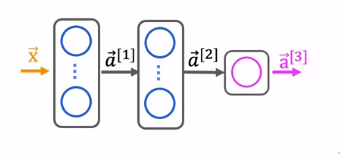
\includegraphics{nn/dense_layer}

Activation value of unit (neuron) $j$ in layer $\ell$

\[ a_j^{[\ell]} = g(\vec{w}_j^{[\ell]} \cdot \vec{a}^{[\ell - 1]} + b_j^{[\ell]}) \]

Input layer is $\ell = 0$.

\subsubsection*{Convolutional layer}

Each neuron only looks at a part of the previous layer's output.

May have faster computation, and needs less training data (less prone to overfitting)

\subsection{Computation graph}

Computes derivatives of neural networks automatically

Assume neural network shown below:

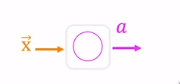
\includegraphics{nn/compgraph-ex/nn}

where:

\begin{align*}
a &= g(z) = z\\
z &= wx + b\\
J(w,b) &= \frac{1}{2} (a-y)^2
\end{align*}

Variables: $w = 2$, $b = 8$, $x = -2$, $y = 2$

\pagebreak

Use forward propagation to calculate cost function

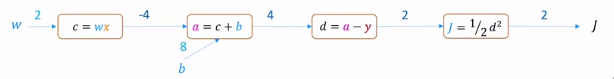
\includegraphics[scale=.8]{nn/compgraph-ex/compgraph}

Computing $\frac{\partial J}{\partial w}$ and $\frac{\partial J}{\partial b}$ will require back propagation.

Start from last node in the graph, and determine how $J$ changes if $d$ changes by some small value $\epsilon$.

\end{document}